\documentclass[11pt]{article}
\usepackage[margin=1.25in]{geometry}
\usepackage{graphicx}
\usepackage{amsmath}
\pdfcompresslevel=9
\pdfobjcompresslevel=2
\begin{document}
\begin{center}
  {\large\bfseries Weight Decay on a Small Data Set}\\[1ex]
  A. Author
\end{center}

\section{Introduction}
A model with many parameters fits a small training set too well: the
training loss keeps falling while the loss on held-out data turns and
rises again. Weight decay is the oldest remedy, and the cheapest one to
try. This note measures how much it helps on a data set of a few hundred
examples, and how the penalty's weight should be chosen.

\begin{figure}[h]
  \centering
  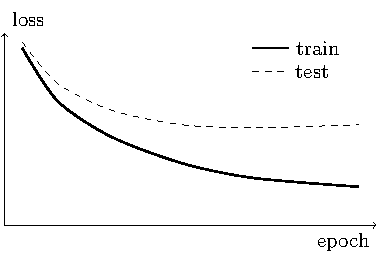
\includegraphics[width=0.55\linewidth]{figures/fig1.pdf}
  \caption{Training and test loss per epoch, without weight decay.}
  \label{fig:loss}
\end{figure}

\section{Method}
We fit a small network to the training set by gradient descent.
The penalty keeps the weights small, which matters when the
training set is small compared with the number of parameters,
as it is in every experiment reported below.
The loss is defined as
\begin{equation}
  L(\theta) = E(\theta)
  + \lambda R(\theta) ,
  \label{eq:loss}
\end{equation}
where $E$ is the squared error of the fit, $R$ the squared norm of the
weights, and $\lambda$ weighs the penalty against the fit.


\section{Results}
Figure~\ref{fig:loss} shows the run without the penalty: after the
fifth epoch the test loss no longer follows the training loss down.
With the penalty of equation~\eqref{eq:loss} the two curves stay
together, and the test loss ends lower by about a fifth.

The weight was chosen on a validation split, from a grid of six values
between one thousandth and one tenth. The best value was the same for
every seed we tried, and the results changed little when it was halved
or doubled, so the choice is not delicate.

Larger data sets need a smaller weight, and the benefit shrinks as the
data set grows: with ten thousand examples the two runs end within a
few hundredths of each other. The penalty is therefore worth its cost
mainly where data are scarce, which is the case this note set out to
study.

A last run kept the penalty but stopped training at the epoch where the
validation loss was lowest. Early stopping alone recovered most of the
gain, and the two together did slightly better than either one, which
agrees with what has been reported for larger models.

\section{Conclusion}
Weight decay is a simple and reliable way to keep a small model from
fitting the noise in a small training set. Its weight can be chosen
coarsely, and it combines well with early stopping. A natural next step
is to see whether the same holds for models whose parameters are
shared across layers, where the penalty acts on fewer weights.
\end{document}
